\documentclass{thesisreport}
\usepackage{todonotes}
\usepackage{parskip}
\usepackage{graphicx}
\usepackage{float}
\usepackage{multicol} %aggiunto da me
\usepackage{enumitem}


\begin{document}

\thispagestyle{empty}

\def\lskip{\vspace{0.5cm}}


\begin{tabular}{p{7cm}p{10cm}}
ÉCOLE CENTRALE DE NANTES
&
\raggedleft UNIVERSITÀ DEGLI STUDI DI GENOVA	% for EMARO students
\end{tabular}

\vspace{2cm}

% EMARO students
\begin{center} \large\sc MASTER ERASMUS MUNDUS \\ \normalsize{EMARO+ ``European Master in Advanced Robotics''} \end{center}


\begin{center}
	2018 / 2019\\
	\lskip
	Master Thesis Report
	\lskip
	
	Presented by \lskip 
	
	Tommaso Elia \lskip
	
	28/12/2018 \lskip\lskip
	
	{\Large \textbf{Dialogue-based interaction processes with smart homes and companion robots}}
	
	\vfill

Jury \lskip
		
	\end{center}
	


\begin{tabular}{p{3cm}p{6cm}p{6cm} }
 President: & Name & Position (Institution) \\ & & \\ 
 Evaluators: & Name & Position (Institution) \\
	      & Name & Position (Institution) \\ 
	      & Name & Position (Institution) \\ & & \\  & & \\ 
  Supervisor(s):  & Fulvio Mastrogiovanni & Assistant Professor (UNIGE)\\
		  & Enrico Reboscio & Project Menager (DotVocal S.r.l.) \\
		  & Renato Zaccaria & Assistant Professor (UNIGE) \\
(EMARO)  & Co-supervisor from M1 & Position, M1 institution 
\end{tabular}

\lskip

\begin{flushleft}
 Laboratory: Laboratoire des Sciences du Numérique de Nantes LS2N
\end{flushleft}

\newpage
\thispagestyle{empty}
\null
\newpage
\addtocounter{page}{-1}
\pagestyle{fancy}
  
 
\section*{Abstract}
   
 Do not forget to check each reference while importing in your Bibtex file.
 Especially, IEEExplore export may lead to ill-formatted conference name like \emph{Robotics and Automation, 
 IEEE International Conference on}.
 
 \newpage
 
 %\section*{Acknowledgements}
 %\newpage
 
\section*{Notations}
 
 \newpage
 
 \section*{Abbreviation}
 
 \begin{tabular}{p{2cm}p{12cm}}
 ADL & Activities of Daily Living\\
 AAL & Ambient Assisted Living \\
 IADL & Instrumental Activities of Daily Living \\
 DS & Dempster - Shafer \\
 DL & Description Logic \\
 SWRL & Semantic Web Rule Language\\
 OWL & Ontology Web Language\\
 EMS & Emergency Medical Services \\
 AR & Activity Recognition \\
 IOT & Internet of Things \\
 ML & Machine Learning \\
 \end{tabular}
 
 \newpage
 
 \listoffigures
 
 \listoftables
 
 \tableofcontents
 
 
 \chapter{Introduction}
 \addcontentsline{toc}{chapter}{Introduction}	 % non-numbered chapters do not appear in table of contents by default

  The growth of the population with progress of medical techniques involve an increase in the number of elderly. Indeed in most of the industrialized countries the demographic and social trends lead to greater elderly among the population. The effects of the trends can be critical for emergency medical services, public and private health care and the individuals themselves. 
 The raising of the average age of the population means an higher number of chronic diseases and therefore also emergency situations. 
 In the district of Kaiserslautern, Germany, a significant study was conducted showing that 44\% of Emergency Medical Services (EMS) are dedicated to elderly above 70 years of age \cite{kleinberger2007ambient}.
 	\begin{figure}[H]
		\centering
		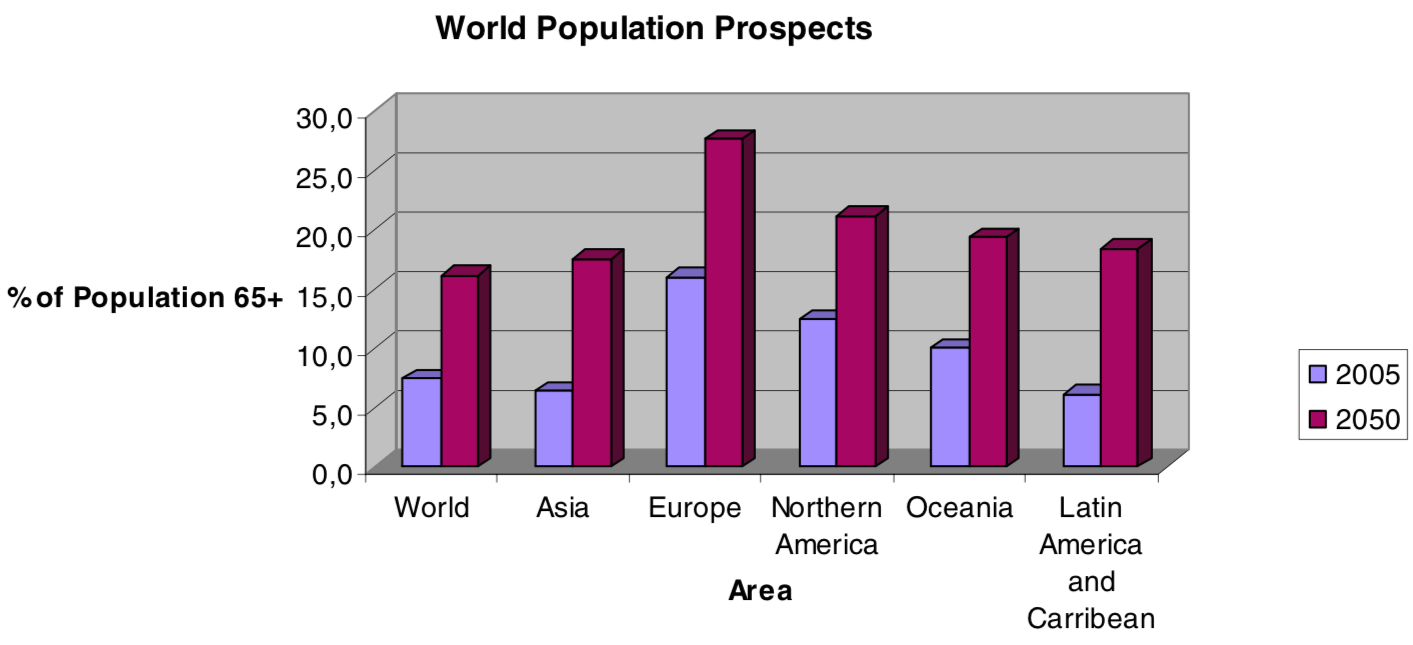
\includegraphics[width=12cm]{Thesis/data/populationProspect.png}
		\caption{\small{Demographical Change according to the United Nations World Population Prospects \cite{kleinberger2007ambient}}}
		\label{fig:populationProspect}
	\end{figure}
 Such a result lead to suppose, decline in service quality or an increase in the cost for such services or both. 
 
 \parskip  \parskip
 
 The Ambient Intelligence technologies help to cope with trends, providing proactive and conscious assistance and supporting the autonomy of the elderly. Indeed Assisted Living solutions, they not only can reduce the costs of managing and monitoring older people but they can also offer better \textit{quality of life} \cite{kleinberger2007ambient}.
 
  To guarantee an improved quality of life it is necessary ensure that the so-colled Activities of Daily Living (ADL) are correctly and regularly performed by the assisted \cite{buoncompagni2017towards}.
 
 As defined \cite{buoncompagni2017towards}, ADL are daily activities related to motion, rest, nutrition, and personal hygiene, which are a qualitative indicator of a person’s wellbeing, determine their quality of life and level of independence. 
 
 Indeed in literature the term smart home is used as synonymous of home based that is context-ware, where context awareness has been defined as: ”having information that can be used to characterize the situation of an entity, where an entity can be a person, place, physical or computational object that is considered relevant to the interaction between a user and an application, including the user and applications themselves” \cite{abowd1999towards}. 

 Now, with giant stride forward in the domain of assistive robots and IOT (Internet of Things) field joined with technological advances in the miniaturization and increased battery life of different types of sensors have given the possibility to create increasingly complex and sophisticated architectures of intelligent environments \cite{phdthesis} \cite{nakashima2009handbook}.
 
 For an easier and immediate comprehension of the possibilities expressible by this type of technology let's have look to some interesting scenario that could support elderly to retrieve their independence:
 \begin{itemize}
     \item \textit{Scenario 1}: The geriatrician with the task of monitoring the health status of elderly could monitor the quality of the patient's sleep through indomitable devices or pressure sensors positioned at the base of the bed, visualizing the pattern of sleep during the night.
     \item \textit{Scenario 2}: The system could monitor the daily activities such as getting out of bed, washing and having breakfast etc. Then it sends an alarm to the geriatrician if, for example, the patient stops eating.
     \item \textit{Scenario 3}: The elder after having woken up decides to take a walk, he puts on his coat and as soon as he crosses the threshold the system realizes that it is probable that it rains and that the elder has not taken the umbrella risking thus to fall ill. Then the system alerts him via a notification on the wearable device or directly via a voice interface.
     \item \textit{Scenario 4}: Let's consider an elderly person who is alone at home  and is heading to the bathroom to wash. The system detects his presence in the bathroom and also receives an unclear signal from the wearable that he wears that could represent a fall by the elderly. To be certain of the elderly safety, the system could verify it  in two ways: it could ask the elderly about his state through a voice interface or it could send a robot 'companion' to check the situation (for example through image analysis - ML).
 \end{itemize}
 
 Smart systems are an inevitable reality but it is important to don't forget to neglect the value of human-human interaction because we do not want that the elderly, inserted in this context, isolates himself from the others \cite{phdthesis}.
 

 \chapter{Background}
This chapter aims to give an overview of the terminologies and basic technologies implemented in any smart environment. \todo{to write somthing more}

 \section{Sensoring}
 An architecture able to monitor these kind of activities can provide very useful information about human behaviour to Human-Robot interaction or cooperation in smart environments \cite{bruno2014public}.  
 
 In literature it is possible to distinguish two different approaches of monitoring: one is based on heterogeneous sensor distributed in an area used to deduce the state of the person inside a context \cite{aggarwal2011human}; the other achieves the information from the wearable devices so sensors located on the person body are able to detect its movements  \cite{bao2004activity}. 
 Therefore we can differentiate two different pivotal concepts:
 \begin{itemize}
    \item to monitor complex sequences of activities reported over time and detected by the interaction with various objects in the monitored area, smart environments are the suggested approach \cite{scalmato2012describing}.
    \item with the advent of the Inertial Measurement Unit (IMU) and therefore the easy monitoring of the acceleration and orientation of limbs, the wearable sensing system, which is also able to monitor bio signals, is certainly the preferred solution to monitor both body gestures and vital signs \cite{bruno2013analysis}.
\end{itemize}
 
Both these approaches are obviously very useful to detect the state of health of the monitored person. They can be used together given that one does not exclude the others. 


\section{Context-Modelling}
 There are several popular context modelling techniques, used in context-aware computing. The context models can be dynamic or static and typically, two different steps, can be distinguished, in representing context according to a model: 
 \begin{itemize}
     \item Context modelling process: when a new context need to be defined in terms of characteristics, attributes, relationships with previously specified context, quality-of context attributes and the queries for synchronous context requests.
     \item Organize context according to the model: the result of the context modelling must be validated, then the new context information needs to be merged and added to to the existing context information repository and finally make available the new context information when required.
 \end{itemize}
 However the parameters and factors considered for the modelling context are very subjective. Indeed there is no standard to specify what type information needs to be considered in the context modelling.
 In \cite{chen2000survey} and \cite{strang2004context} are discussed the most popular context modelling techniques each of which has its own strengths and weaknesses \cite{perera2014context}, synthetically shown In the table below.
 
 	\begin{figure}[H]
		\centering
		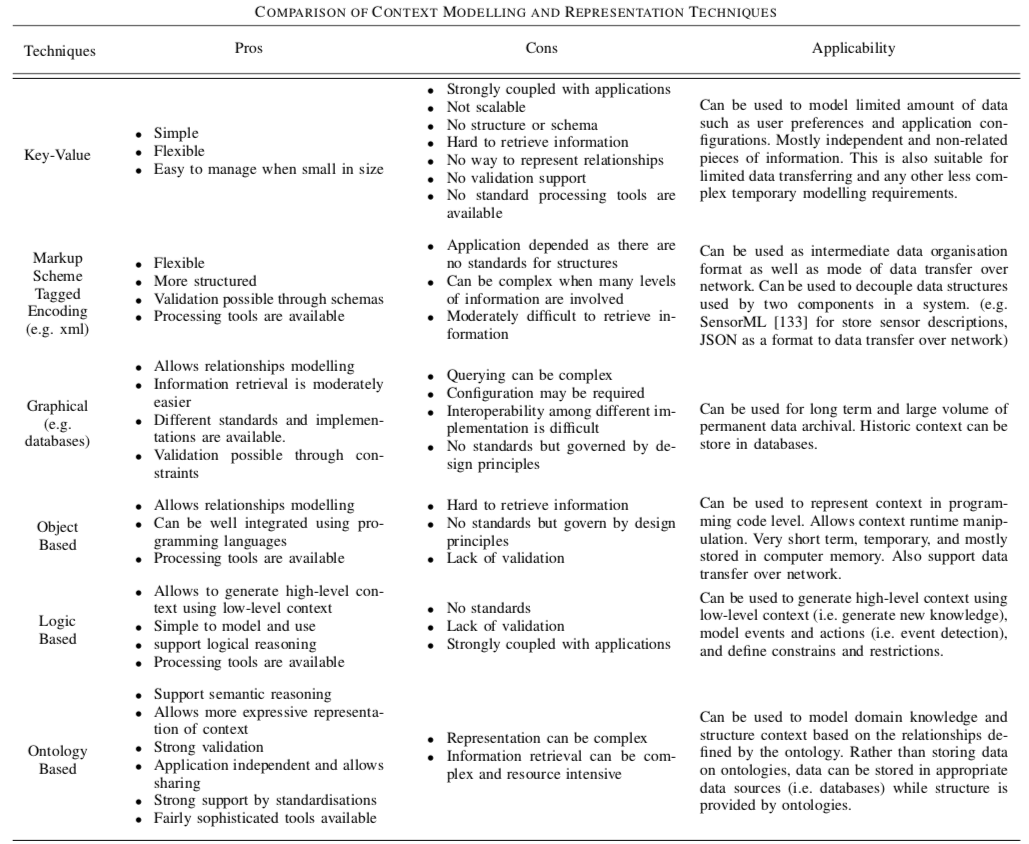
\includegraphics[width=17.5cm]{Thesis/data/ContextModelComparison.png}
		\caption{Comparison of Context Modelling and representation Techniques \cite{perera2014context}}
		\label{fig:populationProspect}
	\end{figure}
 As will be better discussed in the section \ref{ontology} the ontology, according to many surveys, is the preferred mechanism of managing and and modelling context, for all its advantages at the despite its weaknesses \cite{perera2014context}.
 
 
 \subsection{Reasoning}
 The context reasoning, also called inferencing, can be considered as a method to deduct new knowledge based on the available context.  
 it can also be seen as a process to provide hight-level context deduction from a set of contexts \cite{perera2014context}.
 
To recognize the activities, the information from the sensors must be stored and interpreted basis on the model of the context where they came from.  
The modeling procedure has as its aim to create an informative and compact representation of activities. 
We can distinguish two type of the modelling approaches: 
\begin{enumerate}
    \item In logic-based solution, monitoring and recognition of activities is codified through well-defined rules, which are based on ranges of admissible values for a set of relevant parameters. It is often used of for its fast and simple classification procedure (decision trees) \cite{phdthesis}. 
    \item Probability-based solutions assume that the recognition is typically performed by comparing runtime sensory data with the stored models using probabilistic distance measures \cite{phdthesis}. Commonly adopted techniques include Neural Networks \cite{krassnig2010user}, Hidden Markov Mod- els \cite{wiles2012meaning}, \cite{choudhury2008mobile} and Gaussian Mixture Models \cite{bruno2012human}.
\end{enumerate}
In the next sections will be explained in detail. 

\section{Ontology} \label{ontology}

\section{ADL}
Our everyday activities tell us a lot about who we are and to ensure a certain level of independence \cite{buoncompagni2017towards}. For this reason at first it is very important to define them. 
\\
As early as late 1950s, we began to study the psychological, social and biological aspects of aging, analyzing the correlation between human actions and cognitive and motor capabilities \cite{buoncompagni2017towards}. 
\\

From \cite{Multidisciplinary} we can find the Index of activities of Daily Living where show a classification of the functional status of elderly people on the basis of their capability in the execution of 6 different activities in other words called ADLs \cite{buoncompagni2017towards}:
\begin{enumerate}[noitemsep,topsep=1pt,parsep=1pt,partopsep=1pt]
    \item \textit{bathing}
    \item \textit{dressing}
    \item \textit{toileting}
    \item \textit{transferring}
    \item \textit{continence}
    \item \textit{feeding}
\end{enumerate}

But these number of ADL was then extended adding activities deemed relevant for the well-being of a person. These other nine activities, that take the name of Scale of Instrumental ADL \cite{lawton1970assessment} (IADL), require sufficient capabilities of social skills and planning capabilities using and interacting with everyday objects \cite{buoncompagni2017towards}:
\begin{enumerate}[noitemsep,topsep=1pt,parsep=1pt,partopsep=1pt]
    \item \textit{placing a telephone call}
    \item \textit{shopping}
    \item \textit{preparing food}
    \item \textit{housekeeping}
    \item \textit{doing the laundry}
    \item \textit{moving outdoor with public transports}
    \item \textit{moving indoor on foot}
    \item \textit{taking medications}
    \item \textit{handling finances}
\end{enumerate}
Nowadays, as explained in \cite{bruno2014public} the scale of IADL and the index of ADL are the \textit{de facto} standard indexes to evaluate person’s functional status\cite{buoncompagni2017towards}. 

In this essay the term ADL will assume a more general meaning, representing any  considered daily activities. 

\section{Human Activity Recognition}
There are a lot documentations in literature where we discuss of the automatic recognition of ADL. There are often differences about adopted sensing equipment or in the choice of the type of sensors. But typically all the solution share a common paradigm: "\textit{distributed sensing, centralized reasoning}". The sensor information are distributed as raw data, with minimal or no processing, and made available to the reasoning system responsible for analyzing them to extract high level information, the ADL \cite{buoncompagni2017towards}.   

A possible solution is to use binary sensors for their easy interpretation (eg: ON/OFF light switch) and their low cost. However, sensory information must be organized and analyzed in higher-level structures. To do this in literature, the most common and smart solution is to do it with \textit{ontologies} \cite{buoncompagni2017towards}.

\section{Reliability recognition}
The reliability of the recognition is obviously fundamental for any system. Indeed we need to discriminate when a solution is consistent, when all the information is coherent with the specific activities detected, or not, when there are some missing information or contradictory.
As explained in \cite{sentz2002combination} to detailed information about the confidence of the recognition, the reasoning module extends a hierarchy of coarse ontologies implementing the Dempster - Shafer (DS). 

Differently from a broad solution like DS, there are several other system developed specifically to maximize the recognition accuracy of a specific ADL. This kind of solutions are base on one or just a few homogeneous sensors which a imitated number of activities.  

 \chapter{State of the art}
 
%  \section{First topic}
 
%  \section{Second topic}

%  \chapter{Actual work}
  
%  When dealing with rectangled triangles (see Figure \ref{triangle}) I sometimes used this theorem from \cite{pythm001}:
%  \begin{equation}\label{theo}
%   a^2 + b^2 = c^2
%  \end{equation}The demonstration is in Appendix \ref{sec:prooftheorem}.
 
%  \begin{figure}[h]\centering
%   \includegraphics[width=.5\linewidth]{triangle1}
%   \caption{A triangle with letters} \label{triangle}
%  \end{figure}
 
 
%  \chapter{Failed experiments}
 
%  When trying to draw a rectangled triangle, my program comes up with Figure \ref{triangle2} that is neither rectangled nor a triangle.
 
%   \begin{figure}[h]\centering
%   \includegraphics[width=.5\linewidth]{triangle2}
%   \caption{Triangle drawn by my program. Note the 4th side.} \label{triangle2}
%  \end{figure}
 
 
%  \chapter*{Conclusion}
%  \addcontentsline{toc}{chapter}{Conclusion}
 
 
 
%  % switch to A-B-C chaptering
%  \appendix	
 
%  \chapter{Proof of theorem \ref{theo}}
%  \label{sec:prooftheorem}
 
 
%  \begin{proof}
% \eqref{theo} was already demonstrated in \cite{euclides300}.
% \end{proof}
 
 \addcontentsline{toc}{chapter}{Bibliography}

 \bibliographystyle{IEEEtran}
 
 \bibliography{biblio}
 
 
 
 
\end{document}
